\documentclass{article}
\usepackage{ctex} % 加载 ctex 宏包以支持中文
\usepackage{graphicx} % 加载 graphicx 包以支持插入图片
\usepackage{amsmath} % 加载 amsmath 包以支持数学公式
\usepackage{amsfonts} % 加载 amsfonts 包以支持数学字体
\usepackage{amssymb} % 加载 amssymb 包以支持数学符号
\usepackage{hyperref} % 加载 hyperref 包以支持超链接
\usepackage{geometry} % 加载 geometry 包以控制页面布局
\usepackage{algorithm} % 加载 algorithm 包以支持算法环境
\usepackage{algorithmic} % 加载 algorithmic 包以支持算法步骤
\usepackage{bookmark} % 加载 bookmark 宏包以支持书签
\usepackage{tikz} % 加载 TikZ 宏包
\usepackage{pgfplots} % 加载 pgfplots 宏包以支持绘制函数图像

% 设置 pgfplots 的兼容模式
\pgfplotsset{compat=1.18} % 设置 pgfplots 兼容性版本

\begin{document}

\title{\LaTeX TikZ 中文示例} % 文档标题
\author{Raffe Yang}
\date{\today}
\maketitle

\section{简单的线条和形状}

% 绘制一个简单的线条和矩形
\begin{figure}[ht] % 使用 ht 浮动参数
    \centering
    \begin{tikzpicture}
        % 绘制坐标轴
        \draw[->] (-3,0) -- (3,0) node[right] {$x$}; % x轴
        \draw[->] (0,-3) -- (0,3) node[above] {$y$}; % y轴
        
        % 绘制矩形
        \draw[fill=blue!20] (-2,-1) rectangle (1,2);
        
        % 绘制圆
        \draw[fill=red!30] (1,1) circle (1cm);
        
        % 添加标签
        \node at (-1,1) {矩形};
        \node at (1,1) {圆};
    \end{tikzpicture}
    \caption{简单的线条和形状}
\end{figure}

\section{绘制函数图像}

% 绘制函数 y = x^2
\begin{figure}[ht] % 使用 ht 浮动参数
    \centering
    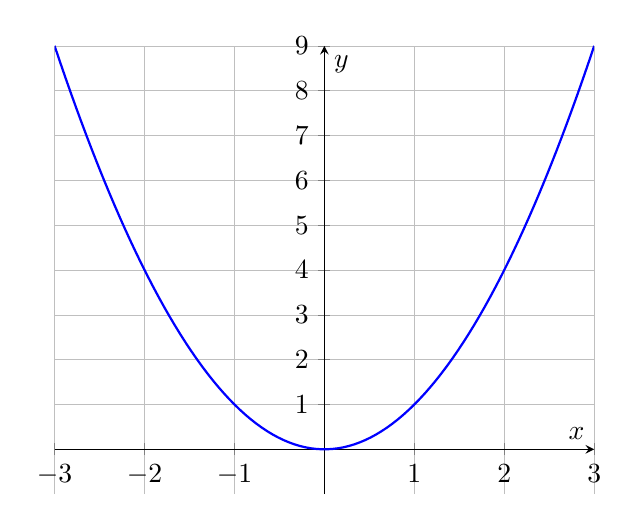
\begin{tikzpicture}
        \begin{axis}[
            axis lines=middle,
            xlabel={$x$},
            ylabel={$y$},
            xmin=-3, xmax=3,
            ymin=-1, ymax=9,
            xtick={-3,-2,-1,0,1,2,3},
            ytick={0,1,2,3,4,5,6,7,8,9},
            grid=both,
            grid style={line width=.1pt, draw=gray!10},
            major grid style={line width=.2pt,draw=gray!50},
            minor grid style={line width=.1pt,draw=gray!20},
        ]
        \addplot[domain=-3:3, samples=100, thick, blue] {x^2}; % 绘制 y = x^2
        \end{axis}
    \end{tikzpicture}
    \caption{绘制函数 $y = x^2$ 的图像}
\end{figure}

\section{绘制复杂图形}

% 绘制一个五角星
\begin{figure}[ht] % 使用 ht 浮动参数
    \centering
    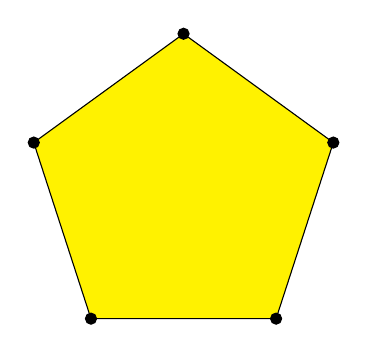
\begin{tikzpicture}
        \draw[fill=yellow] (90:2) -- (162:2) -- (234:2) -- (306:2) -- (18:2) -- cycle; % 五角星
        \foreach \i in {90, 162, 234, 306, 18} % 绘制五角星的顶点
            \draw[fill=black] (\i:2) circle (2pt);
    \end{tikzpicture}
    \caption{绘制一个五角星}
\end{figure}

\end{document}
